\documentclass[tikz,border=2pt]{standalone}
\usepackage{tikz,pgfplots,pgf,calc,fp}
\usetikzlibrary{arrows,decorations.markings,calc}
\usepackage{ifthen}
\begin{document}
\newcommand{\q}{0}
\newcommand{\w}{2}

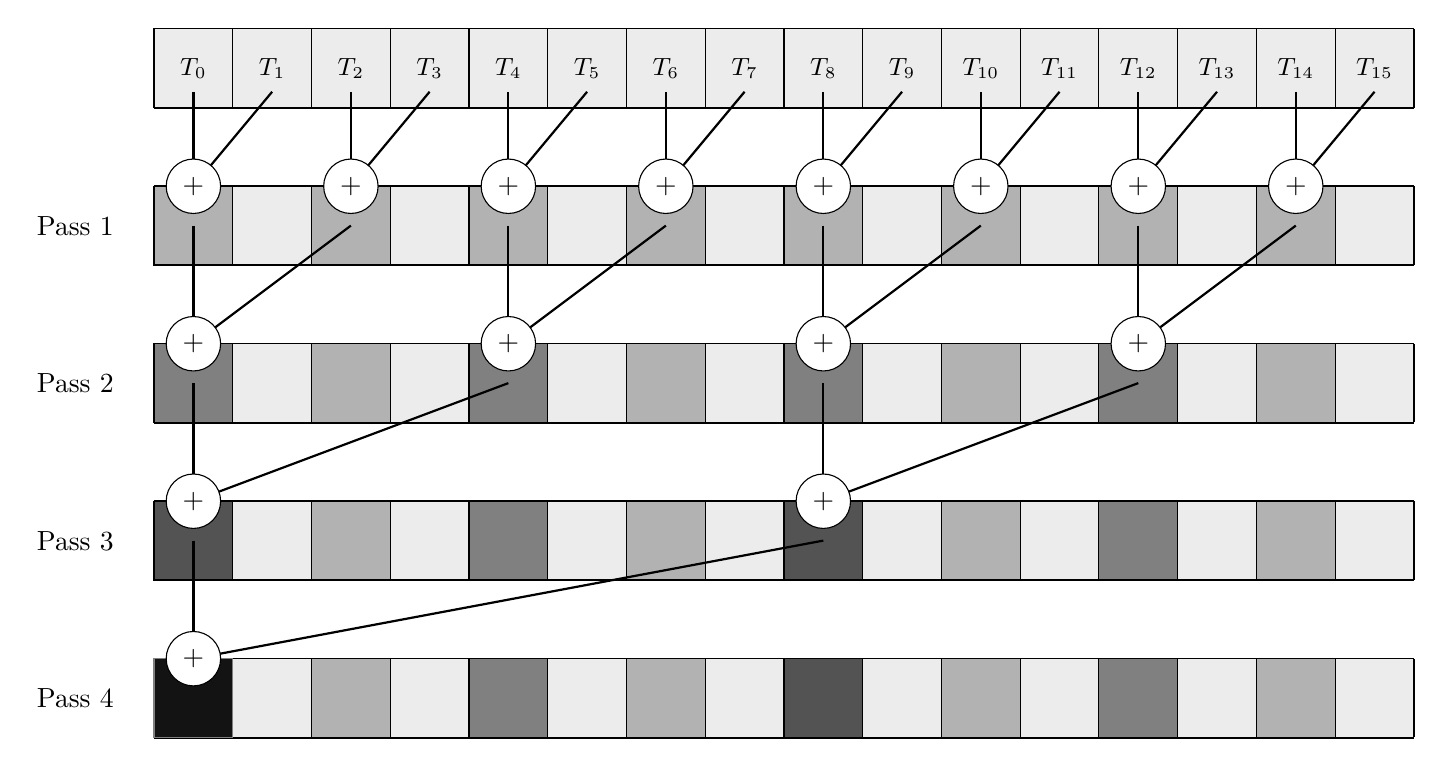
\begin{tikzpicture}[box/.style={rectangle,minimum size=1cm}]
    %\draw[step=1cm, gray, thin,dashed] (0,0) grid (16,16);
    \tikzstyle{filled} = [circle,draw,fill=white,font={}]


\foreach \j in {8,6,4,2,0}{
    \draw [step=1.0, thick] (0,\j) grid (16,\j+1);

    \ifthenelse{\not\equal{\j}{8}}{\node[] at (-1,\j+0.5) {\FPeval{\result}{clip(4-\j/2)}Pass \result};}

    \foreach \i in {0,...,15}{
        \node[box,draw=black,fill=white!85!gray] at (\i+0.5,\j+0.5){};

        \ifthenelse{\equal{\j}{8}}{\node[box,draw=black,fill=white!85!gray] at (\i+0.5,\j+0.5){\small $T_{\i}$};}
    }
}

\foreach \i in {0,2,...,15}{
    \draw[thick,-] (\i+0.5,{8.2}) to (\i+0.5,{7. });
    \draw[thick,-] (\i+1.5,{8.2}) to (\i+0.5,{7. });
    \foreach \j in {6,4,2,0}{
        \node[box,draw=black,fill=white!40!gray] at (\i+0.5,\j+0.5){};
    }
    \node[filled](\i+0.5,{7 }) at (\i+0.5,{7 }) {$+$};
}
\foreach \i in {0,4,...,15}{
    \draw[thick,-] (\i+0.5,{0.5 + 6}) to (\i+0.5,5);
    \draw[thick,-] (\i+2.5,{0.5 + 6}) to (\i+0.5,5);
    \foreach \j in {4,2,0}{
        \node[box,draw=black,fill=gray] at (\i+0.5,\j+0.5){};
    }
    \node[filled](\i+0.5,{5. }) at (\i+0.5,{5. }) {$+$};

}
\foreach \i in {0,8,...,15}{
    \draw[thick,-] (\i+0.5,{0.5 + 4}) to (\i+0.5,3);
    \draw[thick,-] (\i+4.5,{0.5 + 4}) to (\i+0.5,3);
    \foreach \j in {2,0}{
        \node[box,draw=black,fill=gray!65!black] at (\i+0.5,\j+0.5){};
    }
    \node[filled](\i+0.5,{3 }) at (\i+0.5,{3 }) {$+$};


}
\foreach \i in {0}{
    \draw[thick,-] (\i+8.5,{2.5}) to (\i+0.5,1);
    \draw[thick,-] (\i+0.5,{2.5}) to (\i+0.5,1);
    \node[box,draw=gray,fill=gray!15!black] at (\i+0.5,+0.5){};
    \node[filled](\i+0.5,{1 }) at (\i+0.5,{1 }) {$+$};
}
%
\end{tikzpicture}


\end{document}
